\documentclass{standalone}
\usepackage{tikz}
\usepackage{ctex,siunitx,ninecolors}
\setCJKmainfont{Noto Serif CJK SC}
\usepackage{tkz-euclide}
\usepackage{amsmath}
\usetikzlibrary{patterns, calc}
\usetikzlibrary {decorations.pathmorphing, decorations.pathreplacing, decorations.shapes}
\newcommand{\posthead}[2][gray]{
  \begin{scope}[#2]
    \fill[left color=#1,right color= #1,middle color=#1!20](0,0)ellipse(0.05 and 0.02);
    \fill[left color=#1,right color= #1,middle color=#1!20](0.05,0)rectangle(-0.05,0.07);
    \fill[left color=#1,right color= #1,middle color=#1!20](-0.06,0.07)arc(-180:0:0.06 and 0.02)--(0.06,0.15)--(0.05,0.16)--(-0.05,0.16)--(-0.06,0.15)--cycle;
    \fill[#1!50!gray](0,0.16)ellipse(0.05 and 0.02);
    \foreach \x in {75,45,15,-15,-45,-75}
    {
      \draw[very thin,#1!50!gray]({0.05*sin(\x)},{0.16-0.02*cos(\x)})--({0.06*sin(\x)},{0.15-0.02*cos(\x)})--++(0,-0.08);
    }
  \end{scope}
}
\begin{document}
\small
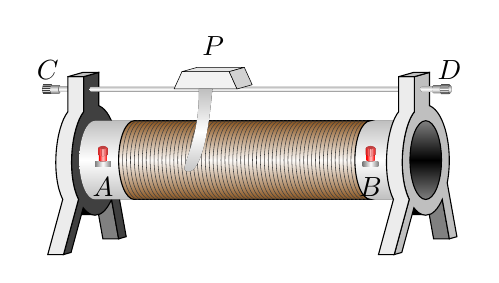
\begin{tikzpicture}[>=latex,scale=1.]
  \fill[top color=gray,bottom color=gray,middle color=white](-2.15,0.9)ellipse(0.02 and 0.06);
  \fill[top color=gray,bottom color=gray,middle color=white](-2.15,0.84)rectangle(-2.05,0.96);
  \foreach \x in {75,45,15,-15,-45,-75}
  {
    \draw[very thin,darkgray]({-2.15-0.02*cos(\x)},{0.9+0.06*sin(\x)})--++(0.1,0);
  }
  \node at (-2.1,0.9)[above]{$C$};
  \fill[gray](-2.05,0.9)ellipse(0.02 and 0.06);
  \fill[top color=gray,bottom color=gray,middle color=white](-2.05,0.9)ellipse(0.02 and 0.05);
  \fill[top color=gray,bottom color=gray,middle color=white](-2.05,0.85)rectangle(-1.95,0.95);
  \fill[gray](-1.95,0.9)ellipse(0.02 and 0.05);
  \fill[top color=lightgray,bottom color=lightgray,middle color=white](-1.95,0.9)ellipse(0.01 and 0.03);
  \fill[top color=lightgray,bottom color=lightgray,middle color=white](-1.95,0.87)rectangle(-1.6,0.93);
  \fill[gray,draw=black](-1.455,-0.692)--(-1.400,-1.000)--(-1.200,-1.000)--(-1.290,-0.500)--cycle;
  \fill[darkgray,draw=black](-1.644, 1.059)--(-1.644, 0.614)..controls(-1.797, 0.425)and(-1.866,-0.181)..(-1.710,-0.500)--(-1.900,-1.200)--(-1.804,-1.173)--(-1.650,-0.606)..controls(-1.619,-0.648)and(-1.568,-0.700)..(-1.500,-0.700)..controls(-1.411,-0.700)and(-1.345,-0.620)..(-1.290,-0.500)--(-1.200,-1.000)--(-1.104,-0.973)--(-1.227,-0.289)..controls(-1.150, 0.109)and(-1.249, 0.607)..(-1.452, 0.691)--(-1.452, 1.114)--cycle;
  \fill(-1.676,-0.700)--(-1.650,-0.606)..controls(-1.619,-0.648)and(-1.568,-0.700)..(-1.500,-0.700)--cycle;
  \fill[lightgray!30,draw=black](-1.844, 1.059)--(-1.844, 0.614)..controls(-1.997, 0.425)and(-2.066,-0.181)..(-1.910,-0.500)--(-2.100,-1.200)--(-1.900,-1.200)--(-1.710,-0.500)..controls(-1.866,-0.181)and(-1.797, 0.425)..(-1.644, 0.614)--(-1.644, 1.059)--cycle;
  \fill[lightgray,draw=black,line join=round](-1.844,1.059)--(-1.644,1.059)--(-1.452,1.114)--(-1.652,1.114)--cycle;
  \fill[top color=lightgray,bottom color=lightgray,middle color=white](-1.5,-0.5)arc(270:90:0.2 and 0.5)--(2.5,0.5)--(2.5,-0.5)--cycle;
  \fill[top color=brown4,bottom color=brown4,middle color=brown9!10,draw=black](-1,-0.5)arc(270:90:0.2 and 0.5)--(2,0.5)arc(90:270: 0.2 and 0.5)--cycle;
  \foreach \x in {-0.95,-0.9,...,1.98} { \draw[very thin,darkgray] (\x,-0.5)arc(270:90:0.2 and 0.5);}
  \fill[left color=gray,right color=gray,middle color=white](-1.5,-0.08)rectangle(-1.3,-0.02);
  \fill[left color=gray,right color=gray,middle color=white](1.9,-0.08)rectangle(2.1,-0.02);
  \fill[top color=lightgray,bottom color=lightgray,middle color=white](-1.55,0.87)arc(270:90:0.02 and 0.03)--(2.4,0.93)--(2.4,0.87)--cycle;
  \draw[fill=lightgray!20,very thin,line join=round](-0.396,1.123)--(-0.496,0.903)--( 0.304,0.903)--( 0.204,1.123)--cycle;
  \draw[fill=lightgray!40,very thin,line join=round](-0.396,1.123)--( 0.204,1.123)--( 0.396,1.177)--(-0.204,1.177)--cycle;
  \draw[fill=lightgray!70,very thin,line join=round]( 0.204,1.123)--( 0.396,1.177)--( 0.496,0.957)--( 0.304,0.903)--cycle;
  \fill[top color=lightgray,bottom color=lightgray,middle color=white](-0.182, 0.903)..controls(-0.163, 0.225)and(-0.446,-0.127)..(-0.341,-0.142)..controls(-0.181,-0.193)and(-0.066, 0.229)..(-0.010, 0.903);
  \fill(2.524,-0.700)--(2.700,-0.700)..controls(2.632,-0.700)and(2.581,-0.648)..(2.550,-0.606)--cycle;
  \fill[gray,draw=black](2.910,-0.500)--(3.000,-1.000)--(2.800,-1.000)--(2.745,-0.692)--cycle;
  \fill[lightgray,draw=black](2.556, 1.059)--(2.556, 0.614)..controls(2.403, 0.425)and(2.334,-0.181)..(2.490,-0.500)--(2.300,-1.200)--(2.396,-1.173)--(2.550,-0.606)..controls(2.581,-0.648)and(2.632,-0.700)..(2.700,-0.700)..controls(2.789,-0.700)and(2.855,-0.620)..(2.910,-0.500)--(3.000,-1.000)--(3.096,-0.973)--(2.973,-0.289)..controls(3.050, 0.109)and(2.951, 0.607)..(2.748, 0.691)--(2.748, 1.114)--cycle;
  \fill[lightgray!30,draw=black](2.356, 1.059)--(2.356, 0.614)..controls(2.203, 0.425)and(2.134,-0.181)..(2.290,-0.500)--(2.100,-1.200)--(2.300,-1.200)--(2.490,-0.500)..controls(2.334,-0.181)and(2.403, 0.425)..(2.556, 0.614)--(2.556, 1.059)--cycle;
  \fill[lightgray,draw=black,line join=round](2.356,1.059)--(2.556,1.059)--(2.748,1.114)--(2.548,1.114)--cycle;
  \fill[top color=gray,bottom color=gray,middle color=black,draw=black](2.7,0)ellipse(0.2 and 0.5);
  \fill[top color=lightgray,bottom color=lightgray,middle color=white](2.65,0.9)ellipse(0.02 and 0.03);
  \fill[top color=lightgray,bottom color=lightgray,middle color=white](2.65,0.87)rectangle(2.8,0.93);
  \fill[top color=gray,bottom color=gray,middle color=white](2.8,0.85)arc(270:90:0.02 and 0.05)--(2.9,0.95)--(2.9,0.85)--cycle;
  \fill[top color=gray,bottom color=gray,middle color=white](2.9,0.84)arc(270:90:0.02 and 0.06)--(3.0,0.96)--(3.01,0.95)--(3.01,0.85)--(3.0,0.84)--cycle;
  \fill[top color=gray,bottom color=gray,middle color=white](3.01,0.9)ellipse(0.02 and 0.05);
  \foreach \x in {75,45,15,-15,-45,-75}
  {
    \draw[very thin,darkgray]({3.01-0.02*cos(\x)},{0.9+0.05*sin(\x)})--({3.0-0.02*cos(\x)},{0.9+0.06*sin(\x)})--++(-0.1,0);
  }
  \node at (3.0,0.9)[above]{$D$};
  \node at (0,1.2)[above]{$P$};
  \posthead[red]{xshift=2cm}
  \posthead[red]{xshift=-1.4cm}
  \node at (-1.4,-0.1)[below]{$A$};
  \node at (2,-0.1)[below]{$B$};
\end{tikzpicture}
\end{document}